\documentclass[aspectratio=169,8pt]{beamer}

\usepackage[T1,T2A]{fontenc}
\usepackage[utf8]{inputenc}
\usepackage[main=russian,english]{babel}
\usepackage[normalem]{ulem}
\usepackage{hyperref}
\usepackage{amsmath,amsthm,amssymb,lmodern}
\usepackage{graphicx} % Allows including images
\usepackage{booktabs} % Allows the use of \toprule, \midrule and \bottomrule in tables
\usepackage{wrapfig}
\usepackage{caption}

\usetheme{Boadilla}
\setbeamertemplate{caption}{\insertcaption}

\title[Проект по дисциплине МИИАД] {Проект по дисциплине "Методы искусственного интеллекта в анализе данных"}
\subtitle{Этап 2}

\author[Бобровских, Иванов, Угадяров] {Бобровских Глеб, Иванов Дмитрий, Угадяров Леонид \\ \tiny\url{https://github.com/ugadiarov-la-phystech-edu/aimda-project}}
\institute{Группа 4}


\begin{document}

\begin{frame}
\titlepage
\end{frame}

\begin{frame}
\frametitle{Набор данных и постановка задачи}

\begin{itemize}
\item { Рассматривается подвыборка за 2014 год из набора данных об убийствах в США \\ Homicide Reports, 1980-2014 --- https://www.kaggle.com/murderaccountability/homicide-reports }
\item Задача прогнозирования временных рядов --- предсказание значений временного ряда (число убийств в США) для 24 месяцев (2013-ый и 2014-ые года) на основе исторических данных \emph {Crime Solved}
\item Метрика качества --- \emph {RMSE} для значений временного ряда
\item {Актуальность --- возможность предсказать количество преступлений в стране на будущий(ие) год(а) кажется вполне очевидной, поскольку качественное решение позволит планировать затраты на полицейские учереждения  }
\end{itemize}

\begin{block}{Признаки}
Number of cases - количество убийств на всей территории США, распределенное во времени 
\end{block}

Количество объектов:  420 (месяцев)\newline

Вклад:
\begin{itemize}
\item Бобровских Глеб --- методы Linear Regression, AutoRegression, ARIMAX
\item Иванов Дмитрий --- нейронные сети
\item Угадяров Леонид --- методы ARIMA, SARIMA, ARIMAX
\end{itemize}

\end{frame}

\begin{frame}
\frametitle{Иллюстрация данных}

Временной ряд: (Ox - количество преступлений, Oy - даты в месяцах)

\begin{figure}[h!]
        \center{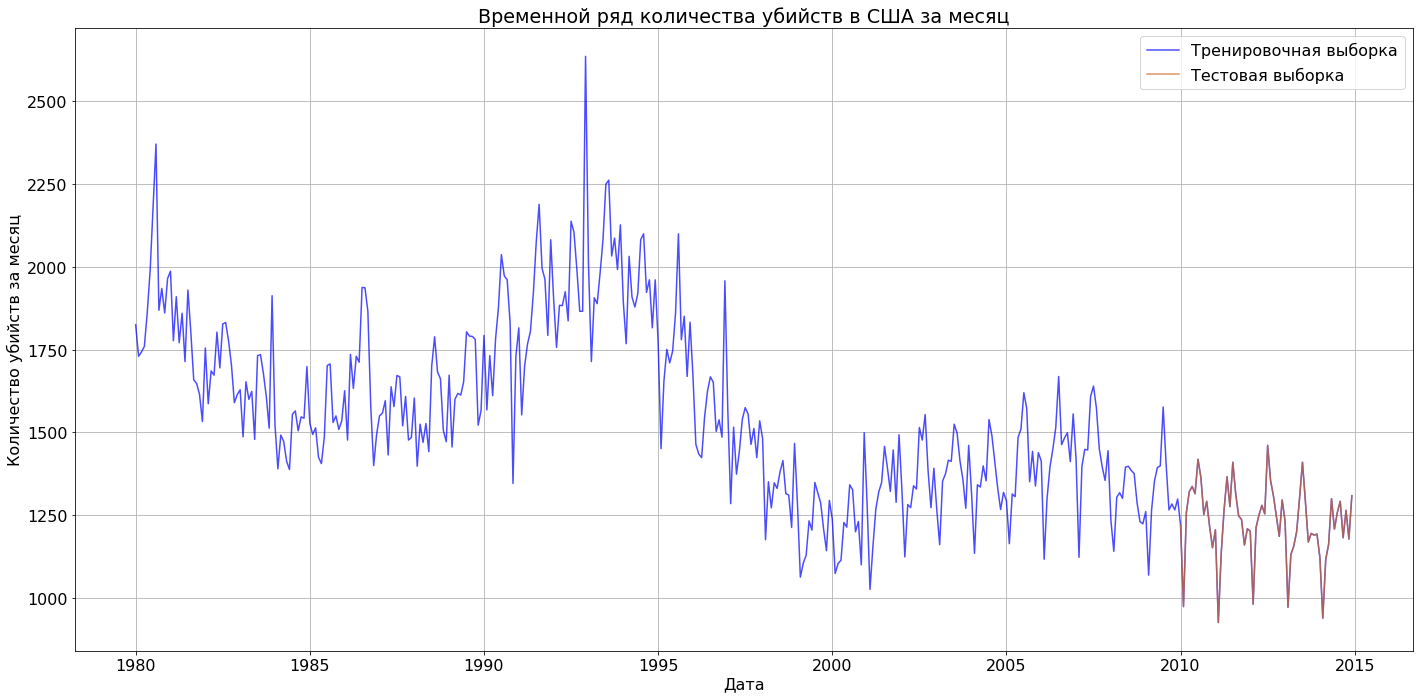
\includegraphics[scale=0.3]{./time_series}}
        \captionsetup{labelformat=empty}
        \vspace{-2.3em}
        \caption[scale=0.25]{}
\end{figure}



Также использовался временной ряд с логарифмированными значениями числа преступлений.

\end{frame}

\begin{frame}
\frametitle{Применённые модели}
\begin{itemize}
\item Линейная регрессия -- sklearn.linear\_model, обучалась на количестве дней от начальной даты;\\
\item Авто регрессия -- statsmodels.tsa.ar\_model.AutoReg, параметры lags = 12; \\
\item ARIMA -- statsmodels.tsa.arima\_model.ARIMA, параметры order = \(12,0,11\), предсказания строились пошагово для дифференцированного шага с параметром lag = 1; \\
\item SARIMA -- statsmodels.tsa.statespace.sarimax.SARIMAX, параметры order = (11,1,11), seasonal\_order=(12,1,11,12), exog=None;\\
\item ARIMAX -- statsmodels.tsa.statespace.sarimax.SARIMAX, order = (1,1,12), seasonal\_order = (0,0,0,0), exog = \{one-hot признаки: месяц, день недели; бинарный признак: выходной день\};\\
\item Полносвязная нейросеть (FCN) -- pytorch.nn.Linear, использовалось различное количество признаков на скрытом слое, в результатах указаны метрики для n\_hidden = 1024; \\
\item Реккурентная нейросеть  (RNN) -- pytorch.nn.RNN, n\_hidden = 1024; \\
\item LSTM -- pytorch.nn.LSTM, n\_hidden = 1024; \\
\end{itemize}

\end{frame}

\begin{frame}
\frametitle{Результаты экспериментов}

{\fontsize{7.5}{10}\selectfont {
\begin{table}
\centering
\caption{Метрики качества классификации обученных моделей на Test}
\vspace{-5pt}
\begin{tabular}{|c|c|c|c|c|}
\hline
\  & \emph {RMSE} & \emph {Log Data RMSE} & \emph {Time Consumption Train (s)} & \emph {Time Consumption Pred (s)} \\
\hline
\emph {Linear Regression} & 1196.16 & 0.09 & 0.001 & 0.0004 \\
\hline
\emph {AutoRegression} & 83.963 & 0.069 & 0.005 & 0.0015 \\
\hline
\emph {ARIMA} & 184.55 & 0.144 & 99.447 & 0.0075 \\
\hline
\emph {SARIMA} & 184.55 & 0.076 & 562.12 & 0.056 \\
\hline
\emph {ARIMAX} & 92.809 & 0.08 & 5.88 & 0.019 \\
\hline
\emph {FCN} & 109.66 & 0.08 & 0.422 (200 эпох) & -- \\
\hline
\emph {RNN} & 273.82 & 0.175 & 16.357 (2000 эпохи) & --\\
\hline
\emph {LSTM} & 273.81 & -- & 43.974 (2000 эпохи) & -- \\
\hline
\end{tabular}
\end{table}
}}


\textbf{Спецификации рабочих машин:} \\
\begin{itemize}
\item Измерение времени для линейной регрессии и прочих классических методов \\ \textbf{Процессор:} 2,3 GHz Dual-Core Intel Core i5, \textbf{Память}: 8 GB 2133 MHz LPDDR3 \\
\item Измерения времени для нейронных сетей \\ \textbf{Процессор}: Intel Core i-7-8750H CPU @ 2.20GHz, \textbf{Память}: 16834 Mb RAM, \textbf{Видеокарта}: NVIDIA GeForce RTX 2060\\
\end{itemize}

\end{frame}
\frametitle{Спецификации рабочих машин}

\end{document}
